% Figure: Three-step scoring cascade
%
% Pipeline (matches Section sec:eval-pipeline and Appendix app:eval_protocol):
%   Input  ->  (1) Parse  ->  (2) Judge Extract  ->  (3) Re-parse  ->  Output
%               |               |
%               | parsed         | NO_ANSWER  =>  score = 0
%               v               v
%   (deterministic return paths to Output)
%
% Width target: NeurIPS \textwidth (~13.97 cm).
% Restricted palette: darknavy (text/borders), forgisorange (single accent),
%   figsteel (muted secondary), figgreen (success path), panelbg (panel fill).
% Three font sizes only: \scriptsize (titles), \fontsize{5.7}{7.2} (body),
%   \fontsize{5.0}{6} (footnotes).

\documentclass[border=4pt]{standalone}
\usepackage{tikz}
\usepackage{xcolor}
\usepackage{amsmath}
\usepackage{amssymb}

\definecolor{darknavy}{HTML}{122128}
\definecolor{forgisorange}{HTML}{FF5A00}
\definecolor{figsteel}{HTML}{878F92}
\definecolor{figgreen}{HTML}{2A8050}
\definecolor{panelbg}{HTML}{F0F4F8}

\usetikzlibrary{arrows.meta, calc, positioning, fit, backgrounds}

\begin{document}
\sffamily
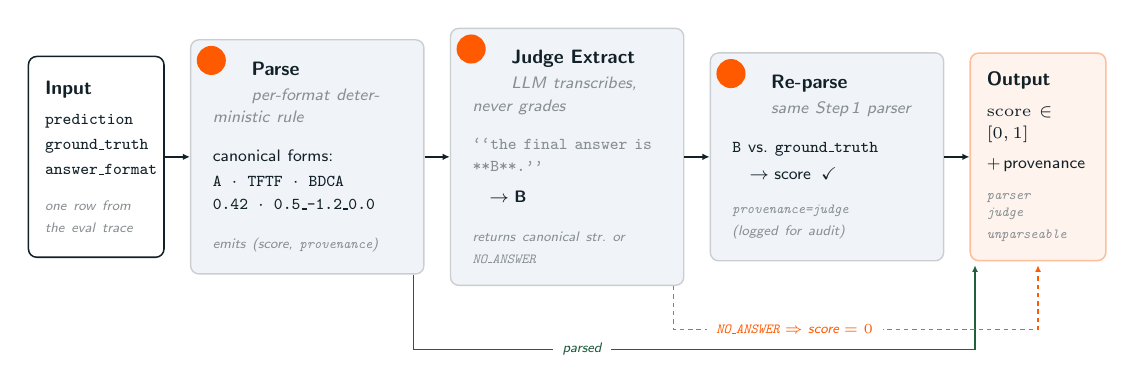
\begin{tikzpicture}[
        font=\sffamily\scriptsize\color{darknavy},
        % --- panel styles ---
        iopanel/.style={
                rectangle, rounded corners=3pt,
                fill=white, draw=darknavy, line width=0.55pt,
                inner xsep=6pt, inner ysep=7pt, align=left,
            },
        steppanel/.style={
                rectangle, rounded corners=3pt,
                fill=panelbg, draw=darknavy!22, line width=0.5pt,
                inner xsep=8pt, inner ysep=8pt, align=left,
            },
        outpanel/.style={
                rectangle, rounded corners=3pt,
                fill=forgisorange!7, draw=forgisorange!40, line width=0.55pt,
                inner xsep=6pt, inner ysep=7pt, align=left,
            },
        % --- arrows ---
        flow/.style={-{Latex[length=2.6pt, width=2.4pt]}, line width=0.7pt, darknavy},
        ok/.style={-{Latex[length=2.4pt, width=2.2pt]}, line width=0.55pt, figgreen!75!black},
        fail/.style={-{Latex[length=2.4pt, width=2.2pt]}, line width=0.55pt,
                forgisorange, dash pattern=on 1.6pt off 1.4pt},
        % --- decorations ---
        stepnum/.style={
                circle, draw=forgisorange, line width=0.5pt, fill=white,
                font=\sffamily\bfseries\fontsize{6}{7}\selectfont, color=forgisorange,
                inner sep=0pt, minimum size=10pt,
            },
        edgelabel/.style={
                font=\sffamily\fontsize{5.5}{6.5}\selectfont\itshape,
                color=figsteel, fill=white, inner xsep=2pt, inner ysep=0.5pt,
            },
        retlabel/.style={
                font=\sffamily\fontsize{5.5}{6.5}\selectfont\itshape,
                inner xsep=1.5pt, inner ysep=0.5pt,
            },
    ]

    % --- LAYOUT CONSTANTS ---
    \def\panelh{2.55cm}     % step panel height
    \def\stepw{2.40cm}      % step panel text width
    \def\iow{1.30cm}        % input/output text width
    \def\hgap{0.32cm}       % horizontal gap between adjacent panels

    % ============================================================
    % INPUT
    % ============================================================
    \node[iopanel, minimum height=\panelh, text width=\iow, anchor=west]
    (input) at (0, 0) {%
        \textbf{Input}\\[3pt]
        {\fontsize{5.7}{7.2}\selectfont\ttfamily prediction}\\[1pt]
        {\fontsize{5.7}{7.2}\selectfont\ttfamily ground\_truth}\\[1pt]
        {\fontsize{5.7}{7.2}\selectfont\ttfamily answer\_format}\\[7pt]
        {\fontsize{5.0}{6}\selectfont\itshape\color{figsteel}one row from\\the eval trace}%
    };

    % ============================================================
    % STEP 1 -- PARSE
    % ============================================================
    \node[steppanel, minimum height=\panelh, text width=\stepw, anchor=west]
    (s1) at ([xshift=\hgap]input.east) {%
        \hspace*{14pt}\textbf{Parse}\\[1pt]
        \hspace*{14pt}{\fontsize{5.7}{7}\selectfont\itshape\color{figsteel}per-format deterministic rule}\\[6pt]
        {\fontsize{5.7}{7.2}\selectfont canonical forms:}\\[1pt]
        {\fontsize{5.7}{7.2}\selectfont\ttfamily A \,$\cdot$\, TFTF \,$\cdot$\, BDCA}\\[0.5pt]
        {\fontsize{5.7}{7.2}\selectfont\ttfamily 0.42 \,$\cdot$\, 0.5\_-1.2\_0.0}\\[6pt]
        {\fontsize{5.0}{6}\selectfont\itshape\color{figsteel}emits (score, \texttt{provenance})}%
    };
    \node[stepnum, anchor=north west] at ([shift={(4pt,-4pt)}]s1.north west) {1};

    % ============================================================
    % STEP 2 -- JUDGE EXTRACT
    % ============================================================
    \node[steppanel, minimum height=\panelh, text width=\stepw, anchor=west]
    (s2) at ([xshift=\hgap]s1.east) {%
        \hspace*{14pt}\textbf{Judge Extract}\\[1pt]
        \hspace*{14pt}{\fontsize{5.7}{7}\selectfont\itshape\color{figsteel}LLM transcribes, never grades}\\[6pt]
        {\fontsize{5.7}{7.2}\selectfont\ttfamily\color{figsteel}``the final answer is **B**.''}\\[3pt]
        \hspace*{6pt}{\fontsize{6.2}{7.5}\selectfont $\rightarrow$\;\textbf{B}}\\[6pt]
        {\fontsize{5.0}{6}\selectfont\itshape\color{figsteel}returns canonical str.\ or \texttt{NO\_ANSWER}}%
    };
    \node[stepnum, anchor=north west] at ([shift={(4pt,-4pt)}]s2.north west) {2};

    % ============================================================
    % STEP 3 -- RE-PARSE
    % ============================================================
    \node[steppanel, minimum height=\panelh, text width=\stepw, anchor=west]
    (s3) at ([xshift=\hgap]s2.east) {%
        \hspace*{14pt}\textbf{Re-parse}\\[1pt]
        \hspace*{14pt}{\fontsize{5.7}{7}\selectfont\itshape\color{figsteel}same Step\,1 parser}\\[6pt]
        {\fontsize{5.7}{7.2}\selectfont\ttfamily B} {\fontsize{5.7}{7.2}\selectfont vs.\ \texttt{ground\_truth}}\\[2pt]
        \hspace*{6pt}{\fontsize{6.2}{7.5}\selectfont $\rightarrow$\;score \,\checkmark}\\[6pt]
        {\fontsize{5.0}{6}\selectfont\itshape\color{figsteel}\texttt{provenance=judge}\\(logged for audit)}%
    };
    \node[stepnum, anchor=north west] at ([shift={(4pt,-4pt)}]s3.north west) {3};

    % ============================================================
    % OUTPUT
    % ============================================================
    \node[outpanel, minimum height=\panelh, text width=\iow, anchor=west]
    (out) at ([xshift=\hgap]s3.east) {%
        \textbf{Output}\\[3pt]
        {\fontsize{6.5}{8}\selectfont $\mathrm{score}\!\in\![0,1]$}\\[3pt]
        {\fontsize{5.7}{7}\selectfont +\,provenance}\\[5pt]
        {\fontsize{5.0}{6}\selectfont\itshape\color{figsteel}\texttt{parser}\\\texttt{judge}\\\texttt{unparseable}}%
    };

    % ============================================================
    % TOP FLOW (sequential cascade)
    % --- inline edge labels are deferred to the caption to avoid
    %     visual collision with adjacent panel borders ---
    % ============================================================
    \draw[flow] (input.east) -- (s1.west);
    \draw[flow] (s1.east) -- (s2.west);
    \draw[flow] (s2.east) -- (s3.west);
    \draw[flow] (s3.east) -- (out.west);

    % ============================================================
    % BOTTOM RETURN PATHS
    % ============================================================
    % Step 1 success -> output (skip judge entirely)
    \draw[ok]
    ([xshift=-4pt]s1.south east) -- ++(0,-0.95) -|
    ([xshift=2pt, yshift=-0.05cm]out.south west);
    \node[retlabel, color=figgreen!70!black, fill=white, inner xsep=2pt]
    at ([xshift=2.0cm, yshift=-0.95cm]s1.south east) {\;parsed\;};

    % Step 2 NO_ANSWER -> output (forces score = 0)
    \draw[fail]
    ([xshift=-4pt]s2.south east) -- ++(0,-0.55) -|
    ([yshift=-0.05cm]out.south);
    \node[retlabel, color=forgisorange, fill=white, inner xsep=2pt]
    at ([xshift=1.4cm, yshift=-0.55cm]s2.south east)
    {\;\texttt{NO\_ANSWER} $\Rightarrow$ score $=0$\;};

\end{tikzpicture}
\end{document}
